%! TEX program = xelatex
%       File: VTthesis_template.tex
%     Created: Thu Mar 24 11:00 AM 2016 EDT
%     Last Change: August 15, 2024
%     Author: Alan M. Lattimer, VT
%	  With modifications by Carrie Cross, Robert Browder, and LianTze Lim. 
%
% This template is designed to operate with XeLaTeX.
%
% All elements in the Title, Abstract, and Keywords MUST be formatted as text and NOT as math.
%
%Further instructions for using this template are embedded in the document. Additionally, there are comments at the end of the file that give suggestions on writing your thesis.  
%
%In addition to the standard formatting options, the following options are defined for the VTthesis class: proposal, prelim, doublespace, draft. 

\documentclass[doublespace,draft,nopageskip]{VTthesis} % nopageskip - Removes arbitrary blank pages.

% Using the following header instead will create a draft copy of your thesis
%\documentclass[doublespace,draft]{VTthesis}

% The lipsum package is just included to put dummy text in the document in order to demonstrate page headers and table of contents behavior. You should remove it once you begin writing your actual thesis or dissertation.
\usepackage{lipsum}
\usepackage{graphicx}

% Title of your thesis
\title{Neuro-Symbolic Reinforcement Learning: Natural Language Driven Multi-Task Agents}

% You should include 3-5 keywords, separated by commas
\keywords{Reinforcment Learning, Neuro-symbolic, Neuro-symbolic Concept Learner, Multi-task Reinforcement Learning, Robotics}

% Your name, including middle initial(s)
\author{Hunter W. Ellis}

% Change this to your program, e.g. Physics, Civil Engineering, etc.
\program{Computer Engineering} 

% Change this to your degree, e.g. Master of Science, Master of Art, etc.
\degree{Master of Science} 

% This should be your defense date:
\submitdate{March 23, 2016} 

% Committee members. Only have five readers and one chair available.
% Only use the ones you need and don't include the ones you don't need.
% You can also declare a Co-advisor. Per the VT ETD standards, 
% you should not include titles such as Dr. or Professor, but can list educational 
% qualifications after the name (i.e., John Doe, MFA or Jane Smith, PhD)
% Names should appear as they do in ESS/Banner/HokieSpa, including middle initials.
\principaladvisor{Thinh T. Doan, PhD}
\coadvisor{Michael S. Hsiao, PhD}
\firstreader{Ryan K. Williams, PhD}
%\secondreader{Kara M. Jones}
%\thirdreader{James Smith}
%\fourthreader{Fourth Committee Member}
%\fifthreader{Fifth Committee Member}

% The dedication and acknowledgement pages are optional. Comment them out to remove them.
\dedication{This is where you put your dedications.}
\acknowledge{This is where you put your acknowledgement.}
%\acknowledge{Thank you to Dr. Thinh Doan and Dr. Michael Hsiao for your guidance and expertise throughout my undergraduate and graduate studies.}

% The abstract is required.
\abstract{
%\abstract{In recent years, neuro-symbolic learning methods have demonstrated promise in tasks requiring a semantic understanding that can often be missed by traditional deep learning techniques. By integrating symbolic reasoning with deep learning architectures the interpretability of the model's reasoning becomes more evident and can provide more control during deployment. This thesis aims to apply neuro-symbolic learning to the domain of reinforcement learning. First, a simulation environment for robotic manipulation tasks based on the Gazebo Harmonic physics simulator and ROS2 middleware suite is presented. In this environment an analysis of policy-gradient based reinforcement learning algorithm is given. Then, by leveraging the performance of deep learning with the semantic reasoning and interpretability of symbolically defined programming, a novel neuro-symbolic learning method is proposed to generalize tasks and motion planning for robotics applications using natural language. This novel neuro-symbolic can be seen as an adaptation of the Neuro-Symbolic Concept Learner (Mao et. al) developed by IBM Watson, in which images and natural language are first processed by convolutional and residual neural networks, respectively and then parsed by a symbolically reasoned program. Where the architecture proposed in this paper differs, is in its use of the Neuro-Symbolic Concept Learner for preprocessing of a given input task, to then inform a reinforcement learning agent of how to act in a given environment. Finally, the novel adaptation of the Neuro-Symbolic Concept Learner is introduced as a method of controlling multi-task agents.
}
%\abstract{\lipsum [1-4]}

% The general audience abstract is required. There are currently no word limits.
\abstractgenaud{
%\abstractgenaud{Neuro-symbolic learning is an area in machine learning that leverages user defined symbolic programming in addition to deep learning. This method goes against the typical approach of end-to-end training of models and instead hopes to benefit from the introduction of symbolic programs.
}

\begin{document}
% The following lines set up the front matter of your thesis or dissertation and are required to ensure proper formatting per the VT ETD standards. 
  \frontmatter
  \maketitle
  \tableofcontents

% The list of figures and tables are now optional per the official ETD standards.  Unless you have a very good reason for removing them, you should leave these lists in the document. Comment them out to remove them.
	\listoffigures
	\listoftables
    \printnomenclature %Creates a list of abbreviations. Comment out to remove it. 

% sample text for abbreviations:
NLP is a field of computer science, artificial intelligence, and linguistics concerned with the interactions between computers and human (natural) languages.
 
\nomenclature{NLP}{Natural Language Processing}
 
$\sigma$ is the eighteenth letter of the Greek alphabet, and carries the 's' sound. In the system of Greek numerals, it has a value of 200. 
 
\nomenclature{$\sigma$}{The total mass of angels per unit area}

% The following sets up the document for the main part of the thesis or dissertation. Do not comment out or remove this line.
	\mainmatter

	%now go ahead and start writing your thesis
	\chapter{Introduction} \label{ch:introduction}
    Neuro-symbolic learning methods and concepts have been used in recent years to achieve results that standalone deep learning and symbolic programming methods have not been able to achieve. [EXAMPLES]. The emerging developments in the field of neuro-symbolic learning has created opportunities to explore applications and adaptations of these methods. The field of Reinforcement Learning (RL) has also made advances -- demonstrating the paradigms effectiveness in creating agents that can perform complex tasks autonomously. The intersection of these two research areas has led to developments that have allowed agents to perform tasks with with both programatic interpretability and learned performance. [EXAMPLES].
%Copy/paste the code below to add sections and subsections to each chapter. Add your own text to the chapter and (sub)section labels to create custom headings.          
    \section{Objectives} \label{se:objectives}
			\lipsum[2]
			\subsection{A sub-section} \label{ss:this_subsection}
				\lipsum[1-4]
	\section{Applications} \label{se:applications}
	\section{Challenges} \label{se:challenges}
	\section{Contributions} \label{se:contributions}
			\lipsum[1-2]

    \chapter{Background} \label{ch:background}
    \section{Markov Decision Process} \label{se:markov_decision_process}
    \section{Reinforcement Learning} \label{se:reinforcement_learning}
    \section{Neuro-symbolic Architectures} \label{se:neurosymbolic_architectures}
    \section{Sim-to-Real} \label{se:sim_to_real}
        \subsection{Transfer Learning} \label{ss: transfer_learning}
        \subsection{Multitask Learning} \label{ss:multitask_learning}
    \chapter{Neuro-symbolic Reinforcment Learning Model}
    Neuro\\
    \begin{figure}[htb]
        \centering
		    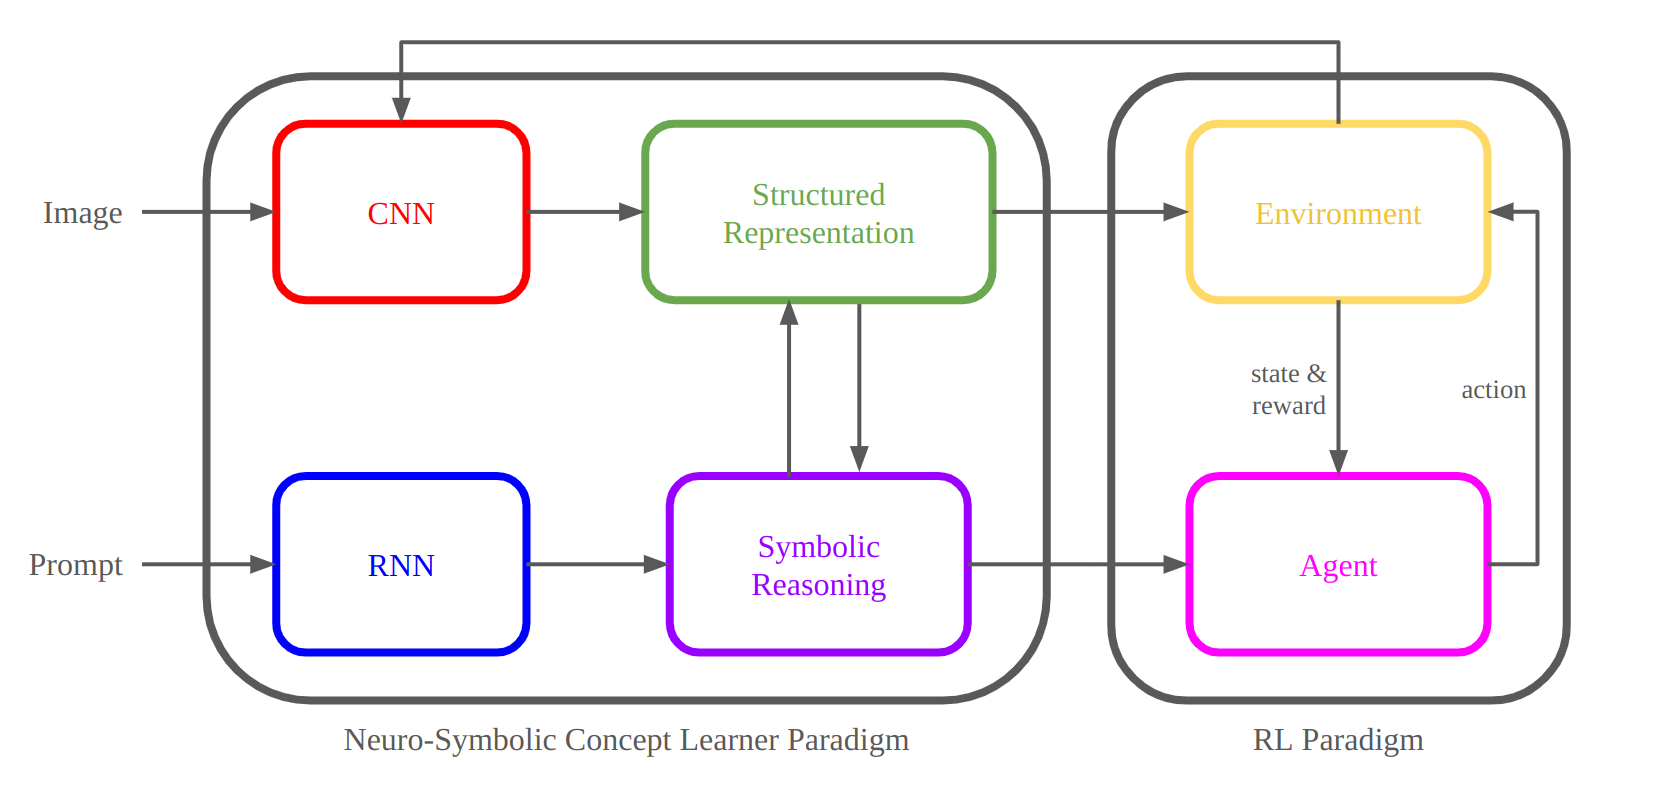
\includegraphics[scale=0.25]{./images/architecture_overview}
				\caption{Overview of proposed architecture.} 
			\label{fig:architecture_overview}
	\end{figure}

    \chapter{Environment and Dataset} \label{ch:training_environment}
    A custom simulation environment was created to demonstrate the possibilities of the Neuro-Symbolic Reinforcement Learning Methods presented in the previous chapter. The environment was set up for basic object manipulation tasks. The cooresponding dataset used to train the model that can be seen as an extension of the CLEVR dataset -- which instead prompts the agent to act on the objects in the environment.
    \section{Environment Overview} \label{ch:environment_overview}
    The environment consists of a six axis robot arm set up in the Gazebo Robotic Simulator. Within the arm's working envelop various basic 3-D shapes (i.e. spheres, cubes, cylinders, etc.) are present.
    
    \section{Robot Operating System} \label{se:robot_operating_system}
    The Robot Operating System is a middleware suite used for robot software development.
    ROS workspaces consist of packages that interface with ROS libraries. 
    \subsection{Description Package} \label{ss:description_package}
    The \texttt{arm\_description} package is a ROS package that contains various files used to describe the physcial characteristics of the robot including its visual, collision, control, and forward kinematics.

    The six-axis robotic arm model deployed in this package is a slightly modified version of an open source six-axis robot design with modfications made to some of the pulleys and end-effector design. The robot arm is made up of six joints (J1-J6) all described as revolute joints in the \texttt{arm\_description}'s Universal Robot Description File (\texttt{.urdf}). Meshes for rendering the robot imported as \texttt{.stl} files and the meshes for collision areas are described by COLLADA (\texttt{.dae}) files. These meshes are linked together in the URDF in a kinematic chain to form the robotic arm manipulator.
    Control of the robot is accomplished through the ROS Jazzy control package.
    \section{Gazebo Robotics Simulator} \label{se:gazebo_harmonic_robotics_simulator}
        Gazebo is a robotic physics simulator developed by Open Robotics which integrates the ODE physics engine, ORGE rendering engine, and support code for sensor and actuator control integration. This environment leverages Gazebo Harmonic (the latest release of Gazebo at the time of writing) to visually render and simulate the physics of the robotic manipulator and the objects in its environment. 
    \subsection{Simulation Package} \label{ss:simulation_package}
    \section{Dataset} \label{se:dataset}
     
	\chapter{Simulations} \label{ch:simulations}

	\chapter{Reality} \label{ch:reality}
	\chapter{Discussion} \label{ch:discussion}
	\chapter{Conclusions} \label{ch:conclusions}

	% This is the standard bibtex file. Do not include the .bib extension in <bib_file_name>.
	% Uncomment the following lines to include your bibliography: 
	%\bibliography{<bib_file_name>}
	%\bibliographystyle{plainnat}   
\end{document}


%****************************************************************************
% Below are some general suggestions for writing your dissertation:
%
% 1. Label everything with a meaningful prefix so that you
%    can refer back to sections, tables, figures, equations, etc.
%    Usage \label{<prefix>:<label_name>} where some suggested
%    prefixes are:
%			ch: Chapter
%     		se: Section
%     		ss: Subsection
%     		sss: Sub-subsection
%			app: Appendix
%     		ase: Appendix section
%     		tab: Tables
%     		fig: Figures
%     		sfig: Sub-figures
%     		eq: Equations
%
% 2. The VTthesis class provides for natbib citations. You should upload
%	 one or more *.bib bibtex files. Suppose you have two bib files: some_refs.bib and 
%    other_refs.bib.  Then your bibliography line to include them
%    will be:
%      \bibliography{some_refs, other_refs}
%    where multiple files are separated by commas. In the body of 
%    your work, you can cite your references using natbib citations.
%    Examples:
%      Citation                     Output
%      -------------------------------------------------------
%      \cite{doe_title_2016}        [18]
%      \citet{doe_title_2016}       Doe et al. [18]
%      \citet*{doe_title_2016}      Doe, Jones, and Smith [18]
%
%    For a complete list of options, see
%      https://www.ctan.org/pkg/natbib?lang=en
%
% 3. Here is a sample table. Notice that the caption is centered at the top. Also
%    notice that we use booktabs formatting. You should not use vertical lines
%    in your tables.
% 
%				\begin{table}[htb]
%					\centering
%					\caption{Approximate computation times in hh:mm:ss for full order 						versus reduced order models.}
%					\begin{tabular}{ccc}
%						\toprule
%						& \multicolumn{2}{c}{Computation Time}\\
%						\cmidrule(r){2-3}
%						$\overline{U}_{in}$ m/s & Full Model & ROM \\
%						\midrule
%						0.90 & 2:00:00 & 2:08:00\\
%						0.88 & 2:00:00 & 0:00:03\\
%						0.92 & 2:00:00 & 0:00:03\\
%						\midrule
%						Total & 6:00:00 & 2:08:06\\
%						\bottomrule
%					\end{tabular}
%					\label{tab:time_rom}
%				\end{table}
% 
% 4. Below are some sample figures. Notice the caption is centered below the
%    figure.
%    a. Single centered figure:
%					\begin{figure}[htb]
%						\centering
%						\includegraphics[scale=0.5]{my_figure.eps}
%						\caption{Average outlet velocity magnitude given an average  
%				        input velocity magnitude of 0.88 m/s.} 
%						\label{fig:output_rom}
%					\end{figure}
%    b. Two by two grid of figures with subcaptions
%					\begin{figure}[htb]
%						\centering
%						\begin{subfigure}[h]{0.45\textwidth}
%							\centering
%							\includegraphics[scale=0.4]{figure_1_1.eps}
%							\caption{Subcaption number one}
%							\label{sfig:first_subfig}
%						\end{subfigure}
%						\begin{subfigure}[h]{0.45\textwidth}
%							\centering
%							\includegraphics[scale=0.4]{figure_1_2.png}
%							\caption{Subcaption number two}
%							\label{sfig:second_subfig}
%						\end{subfigure}
%
%						\begin{subfigure}[h]{0.45\textwidth}
%							\centering
%							\includegraphics[scale=0.4]{figure_2_1.pdf}
%							\caption{Subcaption number three}
%							\label{sfig:third_subfig}
%						\end{subfigure}
%						\begin{subfigure}[h]{0.45\textwidth}
%							\centering
%							\includegraphics[scale=0.4]{figure_2_2.eps}
%							\caption{Subcaption number four}
%							\label{sfig:fourth_subfig}
%						\end{subfigure}
%						\caption{Here is my main caption describing the relationship between the 4 subimages}
%						\label{fig:main_figure}
%					\end{figure}
%
%----------------------------------------------------------------------------
%
% The following is a list of definitions and packages provided by VTthesis:
%
% A. The following packages are provided by the VTthesis class:
%      amsmath, amsthm, amssymb, enumerate, natbib, hyperref, graphicx, 
%      tikz (with shapes and arrows libraries), caption, subcaption,
%      listings, verbatim
%
% B. The following theorem environments are defined by VTthesis:
%      theorem, proposition, lemma, corollary, conjecture
% 
% C. The following definition environments are defined by VTthesis:
%      definition, example, remark, algorithm
%
%----------------------------------------------------------------------------
%
%  I hope this template file and the VTthesis class will keep you from having 
%  to worry about the formatting and allow you to focus on the actual writing.
%  Good luck, and happy writing.
%    Alan Lattimer, VT, 2016
%
%****************************************************************************






